%!Tex Root=**/main.tex
\section{Semantic 3DGS}
\begin{Frame}{Timeline}
	\begin{figure}[htbp]
		% \begin{minipage}[c]{0.20\linewidth}
		% 	\centering
		% 	\resizebox{\linewidth}{!}{
		% 		\begin{tikzpicture}
		% 			\colorlet{0_color_mindmap}{purple!70}
		% 			\colorlet{1_color_mindmap}{green!80}
		% 			\colorlet{2_color_mindmap}{blue!80}
		% 			\colorlet{3_color_mindmap}{red!70}
		% 			\colorlet{4_color_mindmap}{cyan}
		% 			\usetikzlibrary{mindmap}
		% 			\path[mindmap,text=white,
		% 				every node/.style={concept},
		% 				root/.style    = {concept color=um-blue,
		% 						font=\huge\bfseries,text width=12em},
		% 				level 1 concept/.append style={font=\huge\bfseries,
		% 						sibling angle=60,text width=12em,
		% 						level distance=17em,inner sep=0pt},
		% 				level 2 concept/.append style={font=\bfseries,level distance=9em},
		% 			]
		% 			node[root] {Semantic 3DGS}
		% 			[clockwise from=-90]
		% 			child[concept color=0_color_mindmap] { node[concept] {Accuracy} }
		% 			child[concept color=1_color_mindmap] { node[concept] {Efficiency} }
		% 			child[concept color=2_color_mindmap] { node[concept] {Consistency} }
		% 			child[concept color=3_color_mindmap] { node[concept] {Interactivity} };
		% 		\end{tikzpicture}
		% 	}
		% \end{minipage}
		\begin{minipage}[c]{0.75\linewidth}
			\centering
			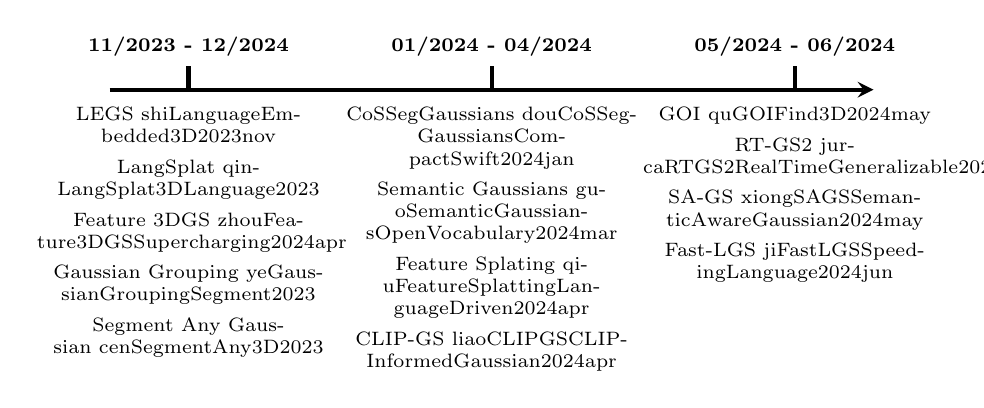
\begin{tikzpicture}
				\usetikzlibrary{calc}

				\pgfmathsetmacro{\dy}{0.3cm/1pt};
				\pgfmathsetmacro{\nodeNum}{3};
				\pgfmathsetmacro{\sepNum}{\nodeNum-1};
				\pgfmathsetmacro{\length}{0.8*\linewidth};
				\pgfmathsetmacro{\edgeLength}{1cm/1pt};
				\pgfmathsetmacro{\dx}{(\length-\edgeLength-\edgeLength)/\sepNum};
				\pgfmathsetmacro{\xShift}{0};

				\tikzset{
					note/.style={
							anchor=north, align=center, text width=\dx, yshift=-\dy/3, font={\scriptsize}
						},
					time/.style={
							anchor=south, font={\scriptsize\bf}
						}
				};

				\coordinate (start) at (0 pt,0 pt);
				\coordinate (end) at (\length pt,0 pt);
				\draw [line width=1.5pt,-stealth] (start) -- (end);

				\foreach \counter in {0,...,\sepNum} {
						\coordinate (s\counter) at (\edgeLength+\counter*\dx pt,0);
						\coordinate (t\counter) at ($(s\counter)+(0,\dy pt)$);
						\draw [line width=1.5pt] (s\counter) -- (t\counter);
					}

				\node [time] at (t0.north) {
					11/2023 - 12/2024
				};
				\node [note] at (s0.south) {
					LEGS~\autocite{shiLanguageEmbedded3D2023nov}\\[1ex]
					LangSplat~\autocite{qinLangSplat3DLanguage2023}\\[1ex]
					Feature 3DGS~\autocite{zhouFeature3DGSSupercharging2024apr}\\[1ex]
					Gaussian Grouping~\autocite{yeGaussianGroupingSegment2023}\\[1ex]
					Segment Any Gaussian~\autocite{cenSegmentAny3D2023}\\[1ex]
					% 2D-Guided 3DGS Seg~\autocite{lan2DGuided3DGaussian2023dec}
				};
				\node [time] at (t1.north) {
					01/2024 - 04/2024
				};
				\node [note] at (s1.south) {
					CoSSegGaussians~\autocite{douCoSSegGaussiansCompactSwift2024jan}\\[1ex]
					Semantic Gaussians~\autocite{guoSemanticGaussiansOpenVocabulary2024mar}\\[1ex]
					Feature Splating~\autocite{qiuFeatureSplattingLanguageDriven2024apr}\\[1ex]
					CLIP-GS~\autocite{liaoCLIPGSCLIPInformedGaussian2024apr}
				};
				\node [time] at (t2.north) {
					05/2024 - 06/2024
				};
				\node [note] at (s2.south) {
					GOI~\autocite{quGOIFind3D2024may}\\[1ex]
					RT-GS2~\autocite{jurcaRTGS2RealTimeGeneralizable2024may}\\[1ex]
					SA-GS~\autocite{xiongSAGSSemanticAwareGaussian2024may}\\[1ex]
					Fast-LGS~\autocite{jiFastLGSSpeedingLanguage2024jun}
				};
			\end{tikzpicture}
		\end{minipage}
	\end{figure}
	\vspace*{\fill}
	\begin{block}{Consensus}
		\par Lift 2D foundation models to 3D scene-specific Gaussians under 2D supervision.
	\end{block}
	\blfootnote{1. 2D foundation models: CLIP, SAM, DINO, etc. }
	\blfootnote{2. Interactivity: manipulation, edit, localization, query, simulation, etc.}
\end{Frame}

\begin{Frame}{Taxonomy}
	\usetikzlibrary{shadows}
	\begin{figure}[htbp]
		\centering
		\resizebox{!}{0.75\textheight}{
			\begin{forest}
				for tree={ my tree },
				[
				\textcolor{um-blue}{\bf Semantic 3DGS}
				[
				\textbf{Accuracy}
				[
					DINO\,\textcolor{blue!70}{\SnowflakeChevron} [\normalfont\autocite{shiLanguageEmbedded3D2023nov,qiuFeatureSplattingLanguageDriven2024apr,douCoSSegGaussiansCompactSwift2024jan}]
				]
				[
					SAM\,\textcolor{blue!70}{\SnowflakeChevron} [\normalfont\autocite{qinLangSplat3DLanguage2023,cenSegmentAny3D2023,zhouFeature3DGSSupercharging2024apr,yeGaussianGroupingSegment2023,liaoCLIPGSCLIPInformedGaussian2024apr,qiuFeatureSplattingLanguageDriven2024apr}]
				]
				[
					3D Prior Regularization [\normalfont\autocite{yeGaussianGroupingSegment2023,cenSegmentAny3D2023}]
				]
				[
					Spatial Feature Fusion [\normalfont\autocite{jurcaRTGS2RealTimeGeneralizable2024may,douCoSSegGaussiansCompactSwift2024jan}]
				]
				[
					3D Segmentation [\normalfont\autocite{guoSemanticGaussiansOpenVocabulary2024mar}]
				]
				]
				[
				\textbf{Efficiency} [
					Dimensionality Alignment [\normalfont\autocite{zhouFeature3DGSSupercharging2024apr,yeGaussianGroupingSegment2023,qiuFeatureSplattingLanguageDriven2024apr}]
				]
				[
					Embedding Compression [\normalfont\autocite{liaoCLIPGSCLIPInformedGaussian2024apr,qinLangSplat3DLanguage2023,jurcaRTGS2RealTimeGeneralizable2024may}]
				]
				[
					Index/Grid Map [\normalfont\autocite{liaoCLIPGSCLIPInformedGaussian2024apr,jiFastLGSSpeedingLanguage2024jun}]
				]
				]
				[
				\textbf{Consistency} [
				Zero-shot Video Tracker\,\textcolor{blue!70}{\SnowflakeChevron}[\normalfont\autocite{yeGaussianGroupingSegment2023,liaoCLIPGSCLIPInformedGaussian2024apr,douCoSSegGaussiansCompactSwift2024jan}]
				][
				Multi-View Association[\normalfont\autocite{jiFastLGSSpeedingLanguage2024jun}]
				][
				Multi-View Self-supervision[\normalfont\autocite{jurcaRTGS2RealTimeGeneralizable2024may}]
				]
				]
				]
			\end{forest}
		}
	\end{figure}
\end{Frame}
\begin{Frame}{Overview}
	\colorlet{easy}{ForestGreen}
	\colorlet{challenging}{Cerulean}
	\colorlet{hard}{OrangeRed}
	\tikzset{
		easy/.style={
				draw=easy,
			},
		challenging/.style={
				draw=challenging,
			},
		hard/.style={
				draw=hard,
			},
	}

	% \par \textbf{For SLAM}: \textcolor{easy-for-slam}{easy}, \textcolor{not-so-easy-for-slam}{challenging}, and \textcolor{hard-for-slam}{hard}.
	\begin{figure}[htbp]
		\centering
		\resizebox{!}{0.75\textheight}{
			\begin{forest}
				for tree={
				my tree
				},
				[
				\textcolor{um-blue}{\bf Semantic 3DGS} [
				\textbf{Accuracy} [
				DINO\,\textcolor{blue!70}{\SnowflakeChevron},challenging [\normalfont\autocite{shiLanguageEmbedded3D2023nov,qiuFeatureSplattingLanguageDriven2024apr,douCoSSegGaussiansCompactSwift2024jan}]
				][
				SAM Feature-based Distillation\,\textcolor{blue!70}{\SnowflakeChevron},challenging [\normalfont\autocite{zhouFeature3DGSSupercharging2024apr,cenSegmentAny3D2023,qiuFeatureSplattingLanguageDriven2024apr}]
				][
				SAM Response-based Distillation\,\textcolor{blue!70}{\SnowflakeChevron},easy [\normalfont\autocite{qinLangSplat3DLanguage2023,yeGaussianGroupingSegment2023,liaoCLIPGSCLIPInformedGaussian2024apr}]
				][
				3D Prior Regularization, easy[\normalfont\autocite{yeGaussianGroupingSegment2023,cenSegmentAny3D2023}]
				][
				Spatial Feature Fusion, challenging[\normalfont\autocite{jurcaRTGS2RealTimeGeneralizable2024may,douCoSSegGaussiansCompactSwift2024jan}]
				][
				3D Segmentation, challenging[\normalfont\autocite{guoSemanticGaussiansOpenVocabulary2024mar}]
				]
				][
				\textbf{Efficiency} [
					Dimensionality Alignment, easy[\normalfont\autocite{zhouFeature3DGSSupercharging2024apr,yeGaussianGroupingSegment2023,qiuFeatureSplattingLanguageDriven2024apr}]
				][
					Index/Grid Map, easy[\normalfont\autocite{liaoCLIPGSCLIPInformedGaussian2024apr,jiFastLGSSpeedingLanguage2024jun}]
				][
					Self-supervised Embedding Compression, hard[\normalfont\autocite{liaoCLIPGSCLIPInformedGaussian2024apr,qinLangSplat3DLanguage2023,jurcaRTGS2RealTimeGeneralizable2024may}]
				]
				][
				\textbf{Consistency} [
					Zero-shot Video Tracker\,\textcolor{blue!70}{\SnowflakeChevron}, easy[\normalfont\autocite{yeGaussianGroupingSegment2023,liaoCLIPGSCLIPInformedGaussian2024apr,douCoSSegGaussiansCompactSwift2024jan}]
				][
					Multi-View Association, easy[\normalfont\autocite{jiFastLGSSpeedingLanguage2024jun}]
				][
					Multi-View Contrastive Learning, hard[\normalfont\autocite{jurcaRTGS2RealTimeGeneralizable2024may}]
				]
				]
				]
			\end{forest}
		}
		\resizebox{0.12\textwidth}{!}{
			\begin{tikzpicture}
				\node [font=\bf] (caption node) {For SLAM};
				\node [my node for tree, draw=easy, below of = caption node] (easy node) {easy};
				\node [my node for tree, draw=challenging, below of = easy node] (challenging node) {challenging};
				\node [my node for tree, draw=hard, below of = challenging node] (hard node) {hard/unattainable};
			\end{tikzpicture}
		}
	\end{figure}
\end{Frame}
